\documentclass{sapthesis}
\usepackage{graphicx}
\usepackage{xcolor}
\usepackage{hyperref}
\usepackage{listings}
\usepackage{todonotes}
\usepackage[backend=biber]{biblatex}

\graphicspath{{img/}}
\addbibresource{Tesi.bib}


\title{Firefox WebExtensions security infrastructure}
\author{Francesco Pasquali}
\IDnumber{1933764}
\course{Laurea triennale in Ingegneria Informatica}
\courseorganizer{Sapienza Università degli studi di Roma}
\AcademicYear{2020/2021}
\advisor{Prof. Emilio Coppa}
\authoremail{pasquali.1933764@studenti.uniroma1.it}
\copyyear{2024}
\thesistype{Tesi triennale}


%% DEFINIZIONI


\newcommand{\MComment}[3]{\textcolor{#3}{ \textbf{#1} \textit{#2}}}
\newcommand{\Nota}[1]{\MComment{Nota:}{#1}{olive}}
\newcommand{\Assert}[1]{\MComment{Assert:}{#1}{red}}

    % Formattazione
\newcommand{\bold}[1]{\textbf{#1}}
\newcommand{\code}[1]{\texttt{#1}}
\newcommand{\file}[1]{\code{#1}}
\newcommand{\method}[1]{\code{.#1()}}
\newcommand{\property}[1]{\code{.#1}}
\newcommand{\attr}[1]{\code{.#1}}
\newcommand{\refSection}[1]{Sezione~\ref{#1}}
\newcommand{\refChapter}[1]{Capitolo~\ref{#1}}
\newcommand{\Sezione}[1]{Sezione~\ref{#1}}
\newcommand{\Capitolo}[1]{Capitolo~\ref{#1}}


    % Utility
\newcommand{\vuln}{\textit{"vuln"}}
\newcommand{\www}{World Wide Web }
\newcommand{\JS}{Javascript }
\newcommand{\JSON}{JSON }
\newcommand{\json}{JSON }
    % Estensioni
\newcommand{\manifest}{\code{manifest.json} }
    % Browser
\newcommand{\idl}{\code{idl} }
\newcommand{\ipdl}{\code{ipdl} }
\newcommand{\AddonManager}{\code{AddonManager} }
\newcommand{\ExtensionProcessScript}{\code{ExtensionProcessScript} }
\newcommand{\WebExtensionPolicy}{\code{WebExtensionPolicy} }
\newcommand{\ContentSecurityPolicy}{\code{ContentSecurityPolicy} }


\definecolor{codegreen}{rgb}{0,0.6,0}
\lstdefinestyle{mystyle}{ 
    commentstyle=\color{codegreen},
    basicstyle=\ttfamily\footnotesize,
    breakatwhitespace=false,         
    breaklines=true,                 
    captionpos=b,                    
    keepspaces=true,                 
    numbers=left,                    
    numbersep=5pt,                  
    showspaces=false,                
    showstringspaces=false,
    showtabs=false,                  
    tabsize=2
}
\lstset{style=mystyle}

%% END DEFINIZIONI

%% ARTICOLO
\begin{document}

%% FRONTE
\maketitle
\tableofcontents
\newpage

%% CONTENUTO

\mainmatter
\chapter{Introduzione}
    \Nota{Perché i browser?}\\
    I Web Browser sono programmi complessi volti a visualizzare contenuti di vario genere
    provenienti dalle fonti piu disparate, dai file locali alle risorse accessibili nell'
    internet, dalle immagini ai linguaggi di scripting.\todo{Qui forse dovresti citare le 
    tecnologie di base dietro ad un browser: HTML, CSS, Javascript, etc.} In un mondo sempre piu connesso, i
    browser sono diventati de facto applicazioni necessarie nella vita di tutti i giorni e
    utilizzate da una vastissima comunità di utenti; la loro diffusione unita alla capacità
    di eseguire codice javascript\todo{direi una mezza frase su cosa e' Javascript} 
    direttamente sulla macchina dell'utente rende i browser
    dei bersagli di interesse per il red-team\todo{Direi non solo red team ma anche in generali attaccanti}, 
    aprendo alla possibilità di compromettere un
    grande numero di dispositivi.\\

    \Nota{Perché Firefox?}\\
    Firefox è un Web Browser che in passato ha avuto un'ampia comunità di utenti, noto per
    le politiche a tutela privacy e la storica concorrenza con Internet Explorer.\todo{E 
    Chrome? Non siamo negli anni 2000!}\todo{Immagino che qui devi ancora espandere per 
    dire che lo hai considerato... e che poi hai scelto di considerare le sue estensioni.}


    \Nota{Perché le estensioni?}\\
    Perché è codice scritto da terze parti a cui il browser da accesso ai contenuti web e
    ad API privilegiato normalmente non accessibili dal DOM\todo{Mi raccomando cerca di accennare, 
    anche se brevemente, ad eventuali concetti (anche se per te sono scontanti ma l'obiettivo 
    di una tesi è far capire a tutti quello che hai studiato.)}, queste caratteristiche mi hanno
    indotto ad astrarre le estensioni come una sorta di ponte tra la pagina e il sistema,
    certo le estensioni non sono le uniche componenti del browser a svolgere questo ruolo
    (basti pensare all'interprete html), ma a differenza delle altre esse sono programmabili
    ( e programmate ) da sviluppatori esterni al progetto Firefox e potenzialmente
    ignari sulle misure di sicurezza nello sviluppo web in ambiente browser. 
    Con questi presupposti ho ipotizzato uno scenario in cui l'attaccante abbia la
    possibilità di sfruttare una estensione vulnerabile ad attacchi di tipo html injection
    e sono andato a studiare se e in che modo il browser sia in grado di difendersi
    da tale scenario.


\chapter{Concetti fondamentali}
\todo{Aggiungi riferimenti alle nuove sezioni \ref{dom} e \ref{webextension-api}}
    Il capitolo fa un escursus\todo{excursus} su definizioni ed elementi utili per la comprensione dei capitoli che seguiranno,
    nella \Sezione{I-linguaggi-fondamentali-del-www} si introducono i tre linguaggi fondamentali del web, HTML5,
    CSS e Javascript al quale dedico la sezione \Sezione{javascript}. CSS verrà soltanto menzionato poiché non ha
    avuto rilievo nella mia ricerca. Seguono due sezioni di presentazione alle estensioni browser, \Sezione{breve_storia_delle_estensioni}
    \todo{e degli attacchi alle estensioni}  è un rapido riassunto sulla storia delle estensioni 
    mentre \Sezione{anatomia_di_una_web_extension} spiega la struttura di una WebExtension.


    \section{I linguaggi fondamentali del \www}
    \label{I-linguaggi-fondamentali-del-www}
        Un Web Browser è un'applicazione capace di richiedere e visualizzare risorse ottenute dalla rete
        all'interno di una finestra.
        Ad oggi un browser deve necessariamente essere in grado di interpretare questi tre tipi di risorsa 
        per rendere il \www fruibile all'utente: documenti HTML5, fogli di stile CSS e script Javascript;
        tutti e tre sono living standards, cioè standard che modificano e aggiornano di anno in anno le
        proprie specifiche.
        HTML5 è un linguaggio di markup che descrive la struttura di una pagina web. Gli elementi della 
        pagina sono rappresentati da tag HTML che talvolta modificano i metadati, la visualizzazione e 
        il comportamento del documento; per esempio il contenuto del tag \code{<script>} può essere interpretato 
        come codice Javascript ed eseguito al volo dal browser, ma lo stesso tag \code{<script>} può anche importare
        uno script da un URL o file sorgente.
        Il frammento di codice nel Listato~\ref{code:esempio-html} è un esempio di utilizzo del linguaggio HTML5, in queste
        righe viene creato un documento che mostra a schermo la scritta "Archive:" ed include tre altre risorse:
        il tag \code{<link>} include e applica alla pagina il foglio di stile \code{page.css} mentre i due tag
        \code{<script>} caricano ed eseguono due script Javascript.
        In Firefox accanto ad HTML5 è presente un altro linguaggio di markup 
        \todo{due parole in piu su XUL}chiamato XUL usato per la UI del browser stesso.

        \begin{lstlisting}[label={code:esempio-html},caption={Un semplice documento html},captionpos=b,language=HTML]
            <!doctype html>
            <html>
                <head>
                    <meta charset="utf-8" />
                    <link rel="stylesheet" href="page.css" />
                    <script src="../shared/archive.js"></script>
                    <script defer src="sbMain.js"></script>
                </head>
                <body>
                    <p>Archive:</p><br/>
                    <section id="output"></section>
                </body>
            </html>
        \end{lstlisting}

    
    \section{Javascript}
    \label{javascript}
        \JS è il linguaggio principe della programmazione web lato frontend. Apparso per la
        prima volta nel 1995 in grembo a Netscape, la sua diffusione ha segnato l'inizio di un \www
        orientato alle applicazioni; ad oggi è usato in numerosi contesti diversi oltre alle pagine web,
        come server in Nodejs o reti neurali in Tensorflow, parti del browser stesso sono programmate
        con \JS. 
        È un linguaggio ad oggetti debolmente tipizzato che supporta la programmazione ad eventi, 
        funzionale, imperativa e la programmazione ad oggetti basata su prototipi \cite{javascript-introduction}.
        Rispetto ad altri linguaggi fortemente orientati alla programmazione oggettuale come Java, in \JS
        gli oggetti si comportano come dizionari, il loro insieme di proprietà può venire espanso, ridotto e 
        modificato a runtime. Tra le proprietà di un oggetto alcune sono rilevanti ai fini del linguaggio:
        \begin{itemize}
            \item \bold{\method{valueOf}} Una funzione che ritorna il "valore" di un oggetto, viene invocata
                    silenziosamente dall'interprete quando l'oggetto è sottoposto ad operazioni logico/matematiche;

            \item \bold{\method{toString}} Una funzione che ritorna la rappresentazione dell'oggetto
                    sottoforma di stringa.

            \item \bold{\attr{\_\_proto\_\_}} È un oggetto che contiene i metodi e gli attributi ereditati, 
                    definisce un \attr{\_\_proto\_\_} a sua volta contenente metodi e attributi della super-super classe 
                    e coì via ricorsivamente. Quando si referenzia la proprietà di un oggetto dapprima la si cerca
                    nell'oggetto stesso e se non viene trovata allora si esplorano ricorsivamente gli oggetti che
                    formano la catena di \attr{\_\_proto\_\_} che termina con il \attr{\_\_proto\_\_} della classe
                    base \code{Object}. È importante sottolineare che il sistema della catena di prototipi non è
                    legato al tipo di oggetto che \attr{\_\_proto\_\_} referenzia, ma dalla sola presenza della chiave 
                    \textit{\_\_proto\_\_} nell'oggetto esplorato e poiché si tratta di una proprietà come le altre
                    \todo{prototype pollution?} è molto facile ridefinirlo.

            \item \bold{\attr{prototype}} Usando la terminologia della programmazione ad oggetti, il \attr{prototype}
                    di una classe contiene i metodi e gli attributi che verranno ereditati da ogni istanza della classe.
                    In realtà in \JS le classi non esistono ma al loro posto ci sono i costruttori, funzioni che creano,
                    inizializzano e ritornano un oggetto che diremo "istanza" del costruttore. Il valore dell'attributo \attr{\_\_proto\_\_}
                    dell'istanza, ovvero l'oggetto prototipale, è un riferimento al \attr{prototype} del costruttore.
            
            \item \bold{\method{constructor}} È il riferimento alla funzione costruttrice dell'oggetto, questa proprietà
                    si trova nel prototipo di un oggetto e viene solitamente usata per verificare l'appartenenza ad una
                    "classe" di oggetti.
        \end{itemize}
        Il listato \ref{code:esempio-javascript-prototype} è un esempio variegato dei concetti introdotti.
        Questo script dichiara un costruttore \code{Letter()} che assegna alle proprie istanze l'attributo \attr{number},
        inoltre tutte le istanze di \code{Letter} ereditano il metodo \method{getNumber}, assegnato al prototipo del costruttore.
        Infine si assegnano alle variabili \code{a},\code{b} e \code{z} tre diverse istanze di \code{Letter}.
        La Figura \ref{fig:javascript-prototype}\todo{tutte le figure devono avere una caption} illustra gli oggetti discussi e i vari riferimenti ai prototipi, \code{Function.prototype}
        è il prototipo per tutti gli oggetti funzione mentre \code{Object.prototype} è il prototipo base di tutti gli oggetti.

        \begin{lstlisting} [
            label={code:esempio-javascript-prototype},
            caption={Frammento di script, viene definito il costruttore \code{Letter} e lo si utilizza per creare tre oggetti },
            captionpos=b
        ]
        function Letter(number) {
            this.number = number;
        }
        
        Letter.prototype.getNumber = function() {
            return this.number;
        };
        
        let a = new Letter(1);
        let b = new Letter(2);
        let z = new Letter(26);
        \end{lstlisting}
        
        \begin{figure}[ht]
            \centering                                                  
            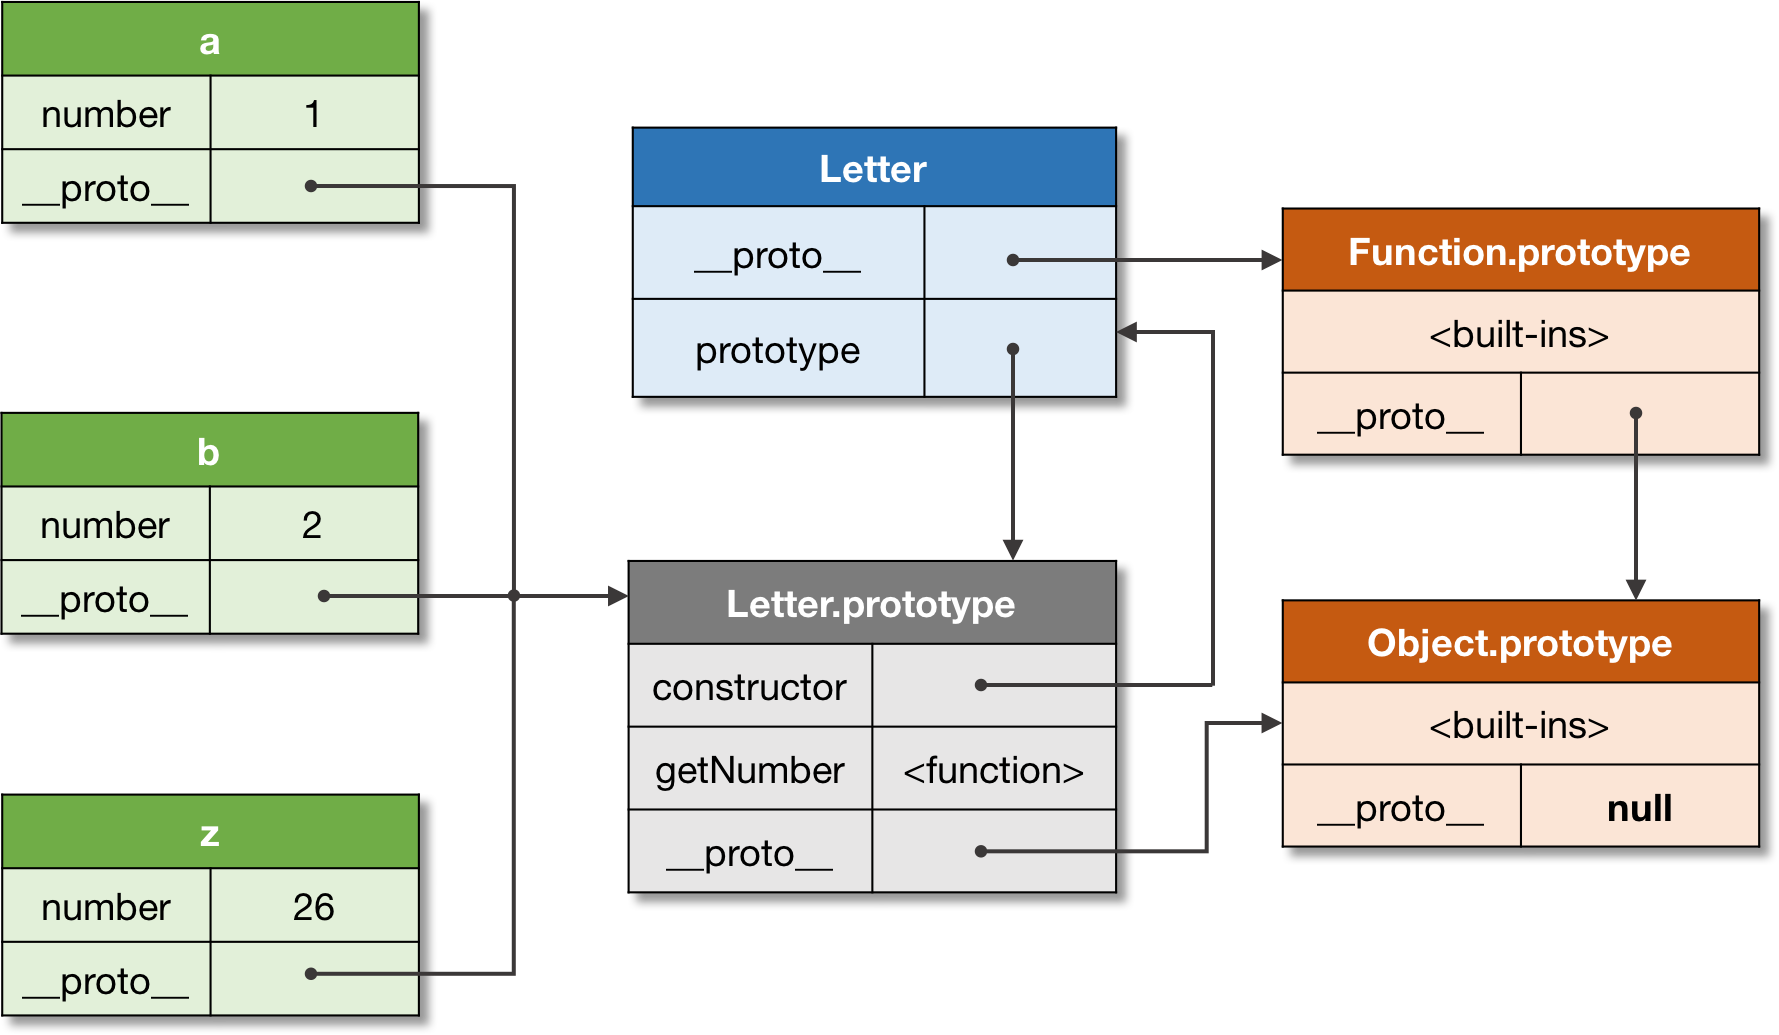
\includegraphics[width=0.5\textwidth]{javascript-constructor.png}
            \caption{}
            \label{fig:javascript-prototype}  
        \end{figure}

    \section{DOM}
    \label{dom}
        Il DOM è la rappresentazione di un documento HTML sottoforma di oggetti \JS \cite{dom-introduction}. 
        Attraverso l'interfaccia offerta dal DOM è possibile modificare programmaticamente gli elementi presenti
        nel documento; tra gli oggetti dichiarati nel DOM \code{document} rappresenta il documento vero e proprio
        mentre \code{window} rappresenta la finestra di visualizzaione che contiene il documento.
        \code{window} ricopre un ruolo molto importante nella programmazione web, esso è l'oggetto globale 
        di tutti gli script eseguiti sulla pagina, ovvero un oggetto che ospita le variabili tra le
        sue proprietà, oltre agli oggetti built-in.

    \section{Breve storia delle estensioni}
    \label{breve_storia_delle_estensioni}
    \todo{attacchi agli applet}
        Le estensioni browser non sono una novità. Già a partire dal 1995 Internet Explorer
        supportava lo sviluppo di plugin \cite{extension-history} affinché visualizzassero contenuti
        dinamici in un World Wide Web fatto di documenti statici, ma è a partire dal 1999 che
        il browser diventa programmabile quando Internet Explorer 4 iniziò a supportare la modifica
        dell'interfaccia utente. Il 2005 vede la nascita di Firefox e l'arrivo degli UserScript,
        piccoli script per la modifica delle pagine web installabili nel browser (precursori dei
        WebExtension Content Script approfonditi nelle prosime sezioni).
        Lo sviluppo di estensioni cross-browser fu per molto tempo una sfida, non c'era uno standard
        comune e ogni browser esponeva questa o quella funzionalità in piu rispetto agli altri; quando
        uscii, Google Chrome non era da meno, ma negli anni la sua ampia diffusione impose lo standard
        de-facto sulla scena; cercando di rimanere al passo con i tempi, Firefox si modificò per
        supportare le estensioni di Google Chrome introducendo il WebExtension framework nel 2017.
        Nonostante le differenze, ad oggi i browser stanno convergendo verso lo stesso formato di estensioni,
        non solo Firefox ma anche Opera e Safari si sono adattati allo standard e sviluppare addon
        cross-browser è diventato possibile.

    \section{Anatomia di una Web Extension }
    \label{anatomia_di_una_web_extension}
        Una estensione è un insieme di script, fogli di stile e documenti html raccolti in una cartella o
        archivio compresso ottenibile dallo store del browser o dai file locali. L'installazione di una
        estensione può essere:
        \begin{itemize}
            \item \bold{built-in}, pre-installata nel browser per migliorare la User Experience
                    o integrare funzionalità utili all'applicazione, l'estensione WebCompat è un esempio;
                    si tratta di una estensione built-in Firefox usata per introdurre fix di compatibilità
                    dopo il rilascio di una nuova versione del browser.

            \item \bold{temporanea}, rimane operativa fintanto che il browser è in esecuzione, ma dovrà essere
                    reinstallata ad ogni avviamento dell'applicazione.

            \item \bold{persistente}, persiste al riavvio dell'applicazione e viene riattivata ad ogni
                    esecuzione del browser.
        \end{itemize}
        
        In ogni estensione che faccia uso del WebExtension framework deve essere presente il file \manifest contenente 
        un oggetto \code{JSON}. Le proprietà dell'oggetto \manifest dichiarano i metadati dell'addon (come nome, 
        versione e descrizione) e le risorse che verranno eventualmente utilizzate.
        Il \manifest può contenere riferimenti a file di altro tipo che modificheranno il comportamento e l'aspetto
        dell'applicazione e si suddividono in:
        \begin{itemize}
            \item \bold{Background}: Sono file che rispondo a eventi del browser, vengono chiamati di background 
                    perché sono eseguiti in modo silenzioso e operano con le componenti interne dell'applicazione.
                    Questi script non possono accedere direttamente alle pagine web.

            \item \bold{Sidebar, popup e option page}: Sono delle interfacce utente introdotte dall'estensione che
                    vengono visualizzate sullo schermo in modo più o meno permanente. Le \textit{sidebar} appaiono sul lato
                    della finestra e rimangono visibili fino alla chiusura manuale da parte dell'utente, i \textit{popup} sono
                    piccole interfacce grafiche disegnate alla pressione di un bottone sulla toolbar o sulla addressbar.
                    La \textit{option-page} è mostrata quando l'utente accede alla pagina di modifica delle preferenze
                    dell'estensione.

            \item \bold{Content script}: Sono script usati per accedere e manipolare le finestre delle pagine web. Si
                    potrebbe dire che sono la controparte UI dei \textit{background} script ma a differenza di questi
                    ultimi non possono interagire con le componenti interne del browser. I \textit{content script} 
                    vengono eseguiti solo sulle pagine che rispettano i criteri di origine specificati nel \manifest{}.
                    A differenza delle pagine web i \textit{content script} possono effettuare richieste cross-domain e
                    usare un piccolo sottoinsieme del WebExtension API.

            \item \bold{Web accessible resources}: Sono risorse di qualsiasi tipo rese accessibili agli altri script
                    dell'estensione.

        \end{itemize}

        La figura \ref{fig:manifest-content} illustra quali file possono essere referenziati per i vari elementi descritti sopra.

        \begin{figure}[ht]
            \centering                                                  
            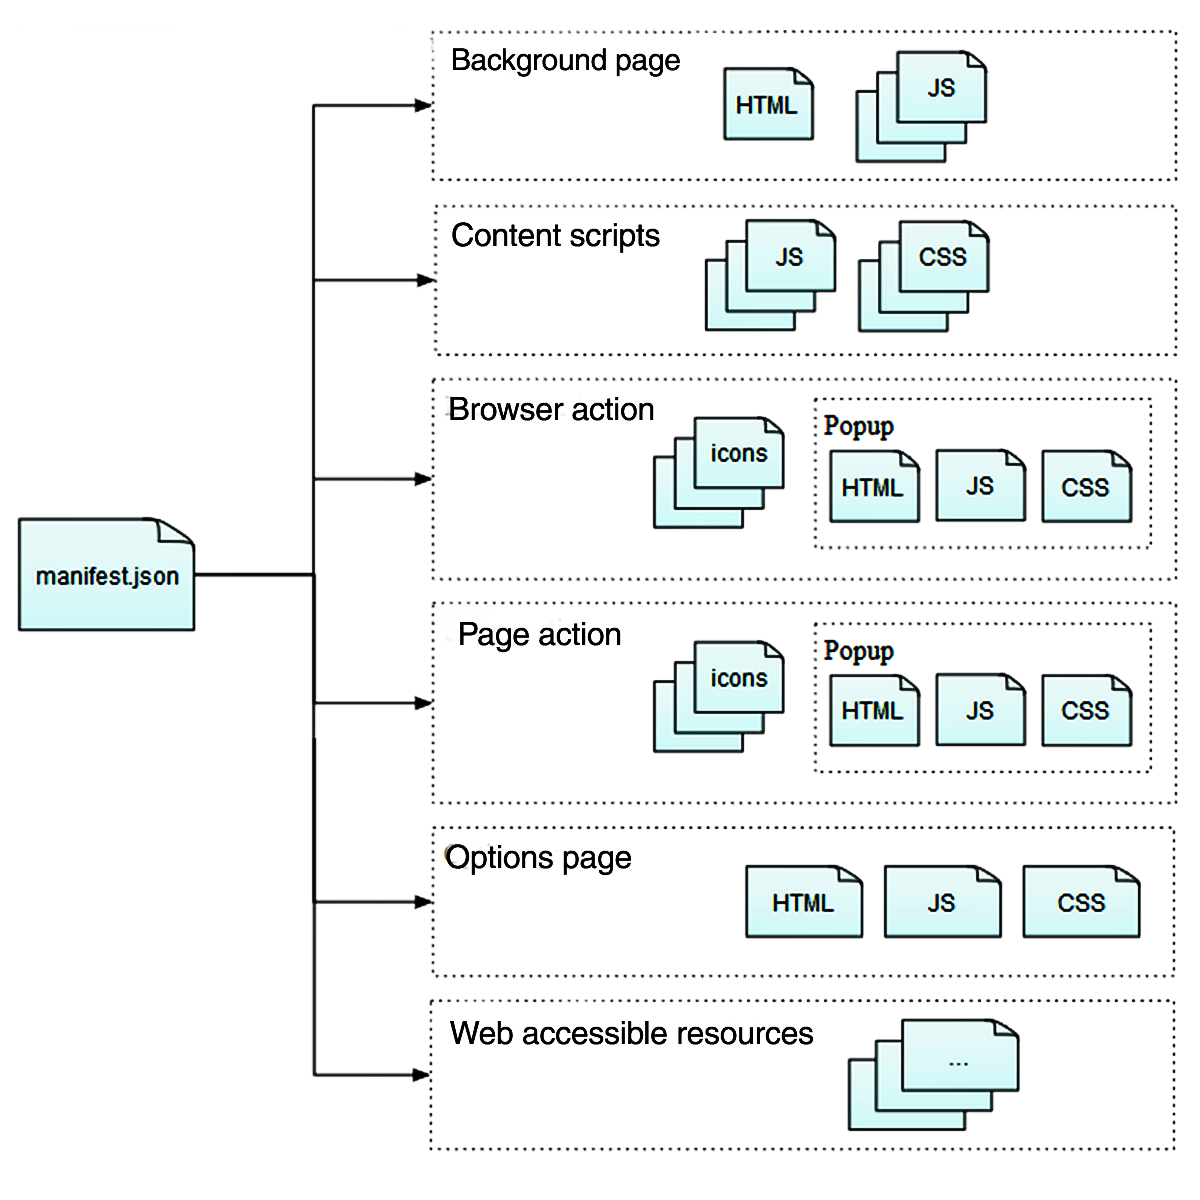
\includegraphics[width=0.5\textwidth]{webextension-manifest-content}
            \caption{Tipi di file referrenziabili dal \manifest }
            \label{fig:manifest-content}                             
        \end{figure}

    \section{Il WebExtension API}
    \label{webextension-api}
        Ogni script \JS può fare uso di funzioni e oggetti messi a disposizione dall'ambiente in cui sta venendo
        eseguito, poiché ogni script ha diverse necessità, l'accesso a queste risorse può venire consentito o negato
        a seconda di quanto il sistema consideri rischioso esporre l'API ad un uso scorretto. Uno script di background
        deve necessariamente poter agire sugli eventi riguardanti il browser nel suo insieme, ma non si può dire lo
        stesso di uno script eseguito in una pagina web, interessato soltanto gli eventi in atto sul suo documento;
        non a caso l'ambiente di esecuzione di background permette di modificare il comportamento del
        browser ma non permette di navigare verso altri URL e specularmente l'ambiente delle pagine web può
        richiedere un sottoinsieme di URI ma non ha alcun accesso agli API del browser.\\
        Il WebExtension framework include nei suoi ambienti l'oggetto \code{browser} (e li suo alias \code{chrome}),
        esso raccoglie un insieme di api utili alle le estensioni e normalmente non accessibili dalle pagine web;
        quali siano questi API dipende dal tipo di script eseguito e dalla voce \code{"permissions"} del \manifest.
        Tra gli api troviamo: \attr{runtime} \cite{browser-runtime} fornisce informazioni riguardo l'ambiente di 
        esecuzione e offre funzioni di messaging, \todo{continua}
    

\chapter{Scenario e ambiente sperimentale}
    Il capitolo descrive i presupposti che hanno guidato la sperimentazione e l'ambiente
    informatico in cui si è svolta. La \Sezione{sec:specifiche-e-piattaforma} è una rapida descrizione
    del sistema informatico usato durante il corso delle ricerche e dell'installazione
    Firefox utilizzata mentre la \Sezione{sec:threat-scenario} illustra il modello di minaccia
    considerato. Infine la \Sezione{sec:estensione-vuln} introduce all'estensione fantoccio 
    bersagliata dagli attacchi, verrà approfondita nel \Capitolo{cap:attaccando-vuln}.

    \section{Specifiche applicazione e piattaforma}
    \label{sec:specifiche-e-piattaforma}
        Per la mia ricerca ho svolto i test utilizzando l'ultima versione corrente di
        Mozilla Firefox v122.0 installata su MacOS Monterey v12.5 con processore Apple M1.
        Il codice sorgente studiato è stato scaricato dalla repository github ufficiale di mozilla,
        commit b59eed0; ogni menzione contenuta in questo articolo è relativa allo stato del codice
        risalente al suddetto commit \cite{mozilla-gecko-dev}. 
        L'applicazione è stata compilata seguendo le istruzioni riportate sul sito ufficiale di mozilla \cite{mozilla-build-firefox}.

    \section{Scenario}
    \label{sec:threat-scenario}
        Per indirizzare la mia ricerca ho deciso di lavorare entro i limiti di uno scenario
        che potesse modellizzare una situazione d'attacco reale in modo quanto più generale e vero-simile.
        Ho definito due attori interessati nella scena, un attaccante e una vittima, e due sistemi
        informatici coinvolti appartenenti a l'uno e l'altro attore.
        L'attaccante è interessato a compromettere il sistema informatico della vittima come parte di 
        una catena di attacco. Il suo obbiettivo è ottenere esecuzione di codice Javascript arbitrario
        al difuori della sandbox in cui il browser Firefox costringe gli script provenienti dal web.
        L'attaccante controlla le risorse di una applicazione web raggiungibile dall'esterno tramite 
        protocollo http/s; che egli abbia o meno controllo sul sistema informatico ospitante l'applicazione
        è indifferente ai fini della ricerca.
        La vittima è un utente privo di competenze in ambito cybersicurezza, è stata persuasa ad utilizzare
        la propria installazione del browser Firefox per navigare sul sull'URL malevolo controllato
        dall'attaccante.
        Il sistema informatico della vittima ospita una istanza del browser Firefox sulla
        quale è stata installata una estensione vulnerabile che è stata rappresentata nel mio ambiente
        di ricerca dall'estensione \vuln di cui si parlerà nella \Sezione{sec:estensione-vuln}.
        L'attaccante non ha alcun modo di accedere o contattare direttamente il sistema informatico della vittima. 


    \section{L'estensione \vuln}
    \label{sec:estensione-vuln}
        Ritenendo che la sola analisi statica del codice sorgente di Firefox non potesse essere
        sufficiente ai fini del mio studio, ho deciso di simulare lo scenario descritto nella
        \Sezione{sec:threat-scenario} creando e installando nel browser una estensione che contenesse
        un qualche errore logico sfruttabile da un potenziale attaccante per tentare di compromettere
        il sistema informatico della vittima.
        Basandomi sulla Top-Ten Owasp delle vulnerabilità nelle applicazioni web \cite{owasp-top-ten}, ho ritenuto
        che l'introduzione di codice vulnerabile ad attacchi di html injection potesse considerarsi uno scenario
        sufficientemente realistico ai fini della mia ricerca.
        Un attacco di html injection consiste nel riuscire ad iniettare ed eseguire codice html nella pagina web
        visualizzata dal browser della vittima; se oltre ad html l'attaccante dovesse riuscisse ad eseguire anche 
        codice \JS allora sarebbe capace di performare attacchi di Cross-Site Scripting aprendo alla possibilità
        di una ancora più profonda compromissione del sistema. Normalmente questo genere di attacchi viene
        attuato sul codice front-end di una applicazione web per abusare delle funzionalità dell'applicazione
        a scapito dell'utente oppure come trampolino verso altre applicazioni (si pensi agli
        attacchi di Cross-Site Request Forgery in cui la pagina vulnerabile viene sfruttata per
        inviare richieste verso una seconda applicazione).\\
        Ogni contesto \JS ha associato un oggetto \code{document}, tra Content Script, Background Script, sidebar,
        popup e pagina opzioni, ogni estensione ha potenzialmente almeno cinque finestre su cui tentare
        html injection, ho scelto di inserire la vulnerabilità nella finestra della sidebar, le ragioni di
        questa scelta sono tre:
        \begin{enumerate}
            \item Il contesto d'esecuzione \JS della sidebar è lo stesso degli script di background, esso espone
                    API che consentono di interagire con vari servizi del browser il che rende la sidebar un
                    bersaglio di alto valore.

            \item Mentre la finestra dei content script è la stessa della pagina in cui stanno venendo eseguiti,
                    invece la sidebar possiede una finestra a sé stante, visualizzabile in qualunque momento e 
                    persistente nella facciata del browser rendendola facile da monitorare.

            \item È un punto che potrebbe verosimilmente contenere codice vulnerabile e raggiungibile dall'attaccante.
                    Trattandosi di una finestra è lecito supporre che venga utilizzata per visualizzare dati raccolti 
                    dall'estensione, dati che devono essere inseriti nel documento html visualizzato.
                    Come gia detto, la finestra può essere aperta solo dall'utente e non
                    è in grado di effettuare richieste verso risorse esterne. In uno scenario verosimile l'ipotetico programmatore
                    di \vuln si sarebbe sentito protetto da queste restrizioni e avrebbe incautamente implementato
                    la logica della UI in modo approssimativo, ignorando i warning dei tool di
                    sviluppo e introducendo codice vulnerabile nel programma.
        \end{enumerate}

        La figura \ref{fig:sidebar-screenshot} mostra la sidebar di \vuln aperta sulla sinistra della pagina
        web controllata dall'attaccante, il riquadro scuro in basso mostra invece il codice html del documento.
        La sidebar sta visualizzando dieci coppie chiave-valore che l'estensione ha estrapolato dal codice
        del sito malevolo, nel \Capitolo{attaccando-vuln}\todo{fix} si approfondirà in che modo l'attaccante sfrutta i
        valori di queste coppie per iniettare codice html.

        \begin{figure}[ht]
            \centering                                                  
            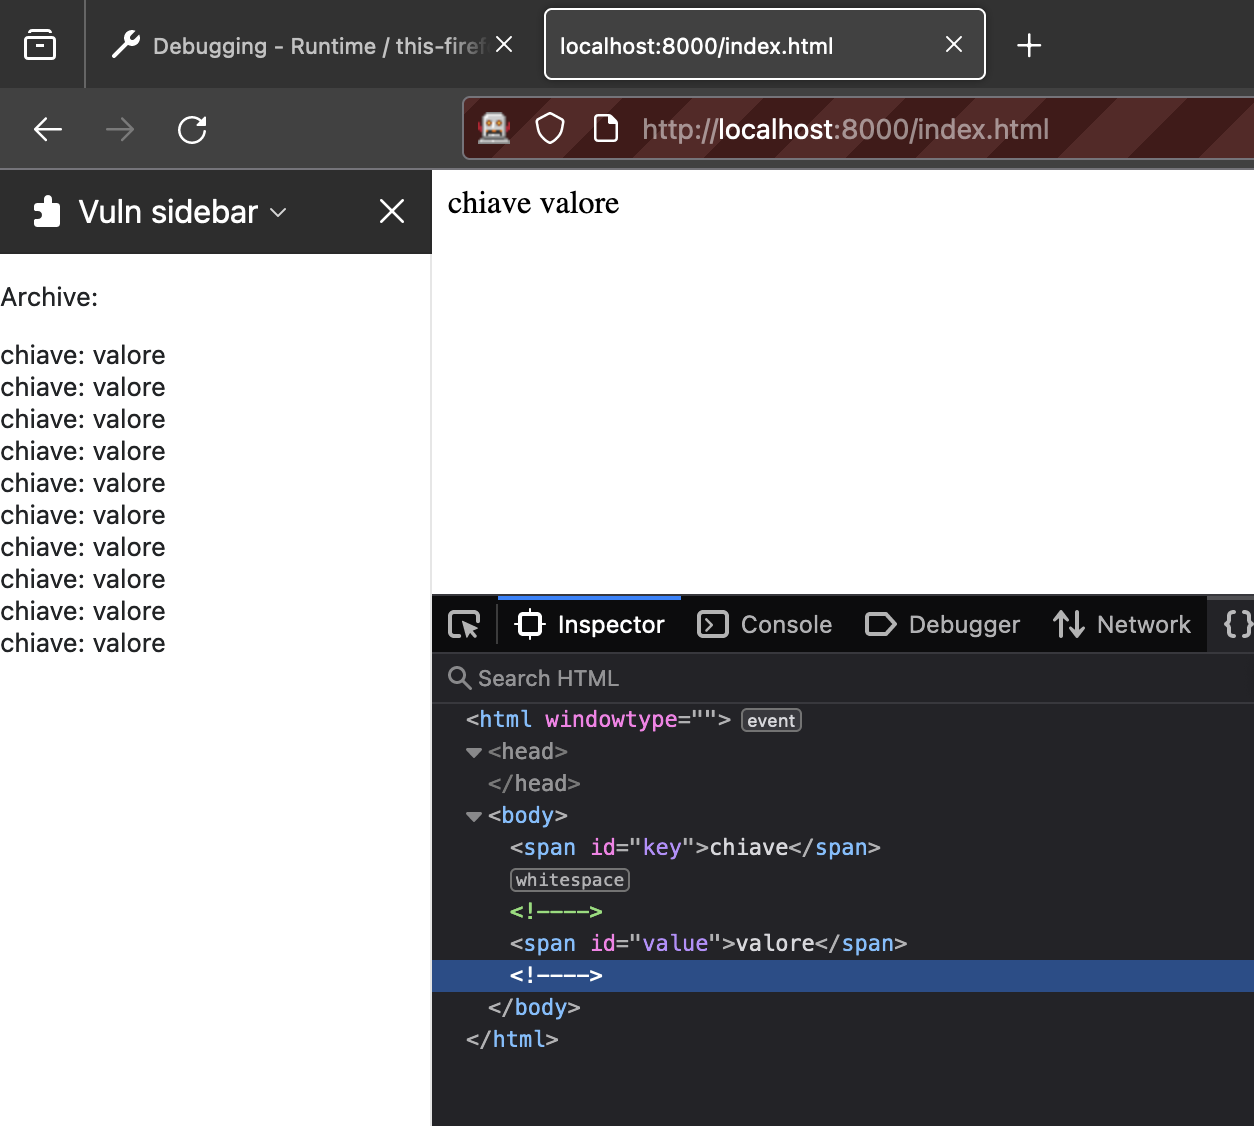
\includegraphics[width=0.5\textwidth]{sidebar-screenshot.png}
            \caption{Visualizzazione della sidebar di \vuln accanto al sito malevolo}
            \label{fig:sidebar-screenshot}                             
        \end{figure}
    

\chapter{L'infrastruttura di sicurezza Firefox}
\label{cap:infrastruttura-sicurezza-firefox}
    Ogni sito internet moderno ha in qualche modo il bisogno di interagire con la rete,
    con uno storage locale, con il file system e con dispositivi audio e video, tutte
    risorse gestite dal sistema operativo, pertanto ogni sito deve poter interagire con
    il sistema operativo della macchina client ma dare questo livello di accesso a codice
    insicuro significa esporre il sistema ad alti rischi di sicurezza per queste ragioni
    il browser deve esporre API che rendano possibili le operazioni richieste dal sito
    senza però compromettere la macchina host.\\
    Firefox non è direttamente responsabile della sicurezza del sistema, questo aspetto è
    invece gestito da rendering engine Gecko di cui Firefox è il front-end.
    Gecko applica quanto detto separando il codice eseguito in compartimenti
    logici, isolati in processi distinti, realizzando layer di separazione a livello
    applicativo e a livello fisico di sistema operativo.

    \section{Modello processi}
        Il codice che compone Firefox e Gecko non è eseguito sotto un unico processo, diversi servizi
        sono eseguiti in diversi processi per garantire solidità nel caso di fallimenti o 
        compromissioni esterne; si dividono in tre categorie:
        \begin{itemize}
            \item \textbf{Parent Process} è il processo principe nonché padre di tutti gli altri,
                è incaricato di coordinare i processi figlio e gestire la comunicazione tra di essi.
                Visualizza pagine ad alti privilegi come \code{about:preferences} e \code{about:config},
                pertanto ospita un ambiente di esecusione ristretto.

            \item \textbf{Helper Processes} sono processi che ospitano servizi, tra essi vi sono servizi
                di interazione con il file system, con la rete, con le immagini e altri ancora.

            \item \textbf{Content Processes} sono processi usati per renderizzare contenuto web, insieme
                al Parent sono gli unici a poter eseguire codice Javascript. Vengono suddivisi in 
                "remote-type", proprietà che specificano i privilegi di accesso agli API.

        \end{itemize}
        Ci sono molti tipi di Content Process di cui due sono di particolare interesse per la mia ricerca:
        \begin{itemize}
            \item \textbf{WebExtensions Content Process}: È utilizzato per caricare pagine
                in background e i subframe delle estensioni web; esiste una sola istanza di
                questo processo ed ha assegnato il remote-type "extension" che garantisce 
                l'accesso al WebExtensionAPI e alla Shared Memory. Tutte le estensioni condvidono
                questo processo e sono visibili tra di loro.

            \item \textbf{Isolated Web Content Process}: Sono usati per ospitare contenuti web attribuiti ad un sito,
                il codice web eseguito in questi processi è considerato insicuro e l'accesso diretto agli
                API di sistema non è permesso. Un nuovo web content viene allocato per ogni sito visitato su
                una browser tab, qualsiasi dominio visitato su una tab differente produce un nuovo processo
                Web Content isolato, invece subframe aperti sullo stesso dominio del superframe contenitore
                vengono eseguiti nello stesso processo del super-frame.
        \end{itemize}

    \section{Sicurezza livello script}
    \label{sec:sicurezza-script}
        Il codice Javascript eseguito da Gecko non proviene solo da fonti terze come pagine web o estensioni,
        l'interfaccia grafica del browser (Firefox) e la logica sono controllati da moduli javascript ad
        alti privilegi di accesso pertanto gli script web non possono eseguire nello stesso ambiente del
        javascript di sistema. Il modello processi in se potrebbe sembrare una soluzione adeguata, ma se
        script web e di sistema dovessero eseguire nello stesso processo si creerebbe un conflitto, inoltre
        il browser deve poter accedere a oggetti del web content; la separazione in processi è troppo 
        restrittiva per questi utilizzi; inoltre Javascript è un linguaggio a tipizzazione debole, funzionale
        e di cui le strutture di supporto alla programmazione ad oggetti sono modificabili, un esempio dei
        rischi introdotti da questa dinamicità sono gli attacchi di prototype pollution\todo{parlane prima, dai citazione}. Il modello di
        separazione dei processi non è sufficiente a gestire proprietà di linguaggio.

        \subsection{Security Policy}
        \label{sec:sicurezza-script-security-policy}
            Una Security Policy è una definizione di che cosa significhi "essere sicuro" per un sistema,
            nel caso di Gecko definisce il livello di accesso garantito verso un oggetto da parte di un
            altro oggetto in relazione a due rapporti: Origine e Privilegi.
            Gli oggetti dotati di stessa "origine" sono detti \code{"same-origin"} e hanno libero accesso
            alle proprietà, oggetti dotati di "origine" differente sono detti \code{"cross-origin"}
            e hanno accesso molto ristretto alle proprietà dell'altro.\\
            Se l'oggetto acceduto si trova in uno scope di privilegio piu basso allora l'accedente avrà
            permessi di accesso libero ma potrà vedere solo un insieme ristretto di proprietà ma se invece
            l'oggetto acceduto dovesse trovarsi in uno scope con privilegi piu alti allora non otterà 
            alcun privilegio di accesso. Script "privilegiati" possono clonare uno o piu oggetti in
            scope meno "privilegiati".

        \subsection{Same-Origin Policy}
            La Same-Origin Policy è un insieme di regole d'accesso a risorse situate su altre "origini".
            L' "origine" di una risorsa è definita come tripla di protocollo, dominio e porta, due risorse
            che condividono la stessa origine sono dette \code{same-origin}, altrimenti \code{cross-origin}.
            Le restrizioni imposte dalla Same-Origin Policy dipendono dal contesto d'uso:
            \begin{itemize}
                \item \textbf{Rete}. Solitamente una risorsa di rete \code{cross-origin} ottiene accesso in
                    scrittura ed embedding mentre la lettura viene proibita, cioé viene reso possibile
                    inviare richieste cross-origin e incorporare risorse esterne ma non è possibile
                    conoscere il contenuto della risposta.
                    Le regole d'accesso di rete \code{cross-origin} possono essere modificate dalla risorsa
                    acceduta tramite header http o tag html \code{meta}.

                \item \textbf{Storage}. Gli spazi di archiviazione sono separati e indipendenti per ogni origine

                \item \textbf{Javascript API}. Due sono gli oggetti visibili a \code{cross-origin}: \code{window}
                    e \code{location}, di questi solo un sottoinsieme di proprietà è accessibile, tra queste
                    sono notevoli \code{.postMessage} di \code{window} che consente di scambiare dati \code{cross-origin}
                    tra gli script e \code{.href} di \code{location}, accessibile solo in scrittura, permette di
                    redirigere la finestra.
            \end{itemize}

            \subsubsection{Eccezioni}
                Non tutti i protocolli vengono trattati allo stesso modo dalla Same-Origin Policy, le risorse
                caricate da \code{about:blank} o \code{javascript:} sono considerate avere la stessa origine del
                documento che le contiene, mentre l'origine \code{file:///} è trattata come origine opaca cioè
                le risorse ottenute con questo protocollo non sono mai considerate same-origin, nemmeno se
                risiedenti nella stessa directory.

            \subsubsection{Iframe pitfall}
            \Nota{Rimuovere?}\todo{Se non e' funzionale al discorso che fai dopo, puoi anche rimuoverla}
                L'implementazione degli iframe risente di una piccola falla di referenza; quando viene inserito
                nel documento, \code{iframe} incorpora la pagina \code{about:blank} che viene sostituita non
                appena la risorsa è caricata, pertanto lo stesso iframe mostra agli API javascript oggetti con
                origine differente in due momenti diversi.


        \subsection{Compartimenti Javascript}
            I compartimenti sono aree di memoria indipendenti e sono alla base della sicurezza degli script
            in Gecko; ogni oggetto globale e gli oggetti associati alle sue proprietà condividono lo stesso
            compartimento. Gli oggetti memorizzati in un compartimento non sono direttamente accessibili da 
            script appartenente ad un compartimento diverso, la condivisione di oggetti è ottenuta tramite
            oggetti wrapper memorizzati nel compartimento dello script che referenziano l'oggetto originale,
            il grado di accesso fornito dal wrapper verso l'oggetto rappresentato è determinato da Gecko
            secondo la Security Policy.
            I criteri di origine sono valutati considerando come "origine" l'url dell'istanza di \code{window}, 
            che è oggetto globale di ogni compartimento. I criteri di privilegio sono invece determinati
            secondo l'Entità di Sicurezza del compartimento.
            \begin{itemize}
                \item \textbf{Same-Origin.} È il caso più comune, all'oggetto accedente viene concesso un
                    wrapper trasparente che garantisce accesso completo all'oggetto richiesto come se 
                    fosse parte dello stesso compartimento. 

                \item \textbf{Cross-Origin.} Gecko assegna un wrapper cross-origin che limita l'accesso 
                    secondo la Same-Origin Policy.

                \item \textbf{Privilegio Maggiore.} Se lo scope acceduto ha privilegi minori, allora si
                    ottiene un wrapper Xray (di più su Xray Vision in seguito\todo{metti ref al punto esatto})

                \item \textbf{Privilegio Minore.} Se lo scope acceduto ha privilegi maggiori, allora si
                    ottiene un wrapper opaco che nega l'accesso all'oggetto.
            \end{itemize}

        \subsection{Entità di Sicurezza}
        \label{sec:security-principal}
            Un Entità di Sicurezza è qualunque entità che puo essere autenticata da un sistema, in Gecko
            esistono quattro entità sulle quali è definita una relazione di sicurezza.
            Per determinare il rapporto tra due entità si verifica se ciascuna sussume l'altra.
            Le quattro entità sono:
            \begin{itemize}
                \item \textbf{Entità di sistema.} Supera ogni check di sicurezza, sussume sè stessa e
                    tutte le altre entità. I compartimenti che eseguono codice di sistema sono istanze
                    di questa entità.

                \item \textbf{Entità di Contenuto.} È associata ai contenuti web ed è definita 
                    dall'origine del contenuto, sussume ogni altra entità con cui condivida
                    l'origine.

                \item \textbf{Entità Espansa.} È definita come una lista di "origini" su cui si ha accesso
                    completo, essa sussume ogni entità che abbia inclusa la propria origine nella lista
                    ma non è sussunta da nessuna di esse.
                    Un esempio di impiego delle entità espanse sono i Content Script delle estensioni che
                    possono accedere al contenuto di più pagine ma non viceversa. In generale l'entità
                    espansa è utilizzata per garantire permessi cross-origin allo script senza però
                    renderlo entità di sistema.

                \item \textbf{Entità Nulla.} Fallisce quasi tutti i check e non sussume sè stesso, può
                    essere acceduto solo da un'entità di sistema.
            \end{itemize}
            Le entità non modellizzano solo il livello di privilegio del compartimento ma anche l'origine
            el il test di relazione fornisce le informazioni sufficienti a computare un wrapper secondo
            la Security Policy, infatti se un compartimento sussume l'altro allora deve avere privilegi pari
            o maggiori, se entrambi si sussumano allora sono \code{same-origin}, se nessuno sussume allora
            si tratta di un accesso \code{cross-origin} se invece è uno solo dei due a sussumere allora
            vi è una differenza di privilegi. L'algoritmo di decisione impiegato da Gecko è rappresentato
            in questo grafico:
            \begin{figure}[ht]
                \centering                                                  %% centrata
                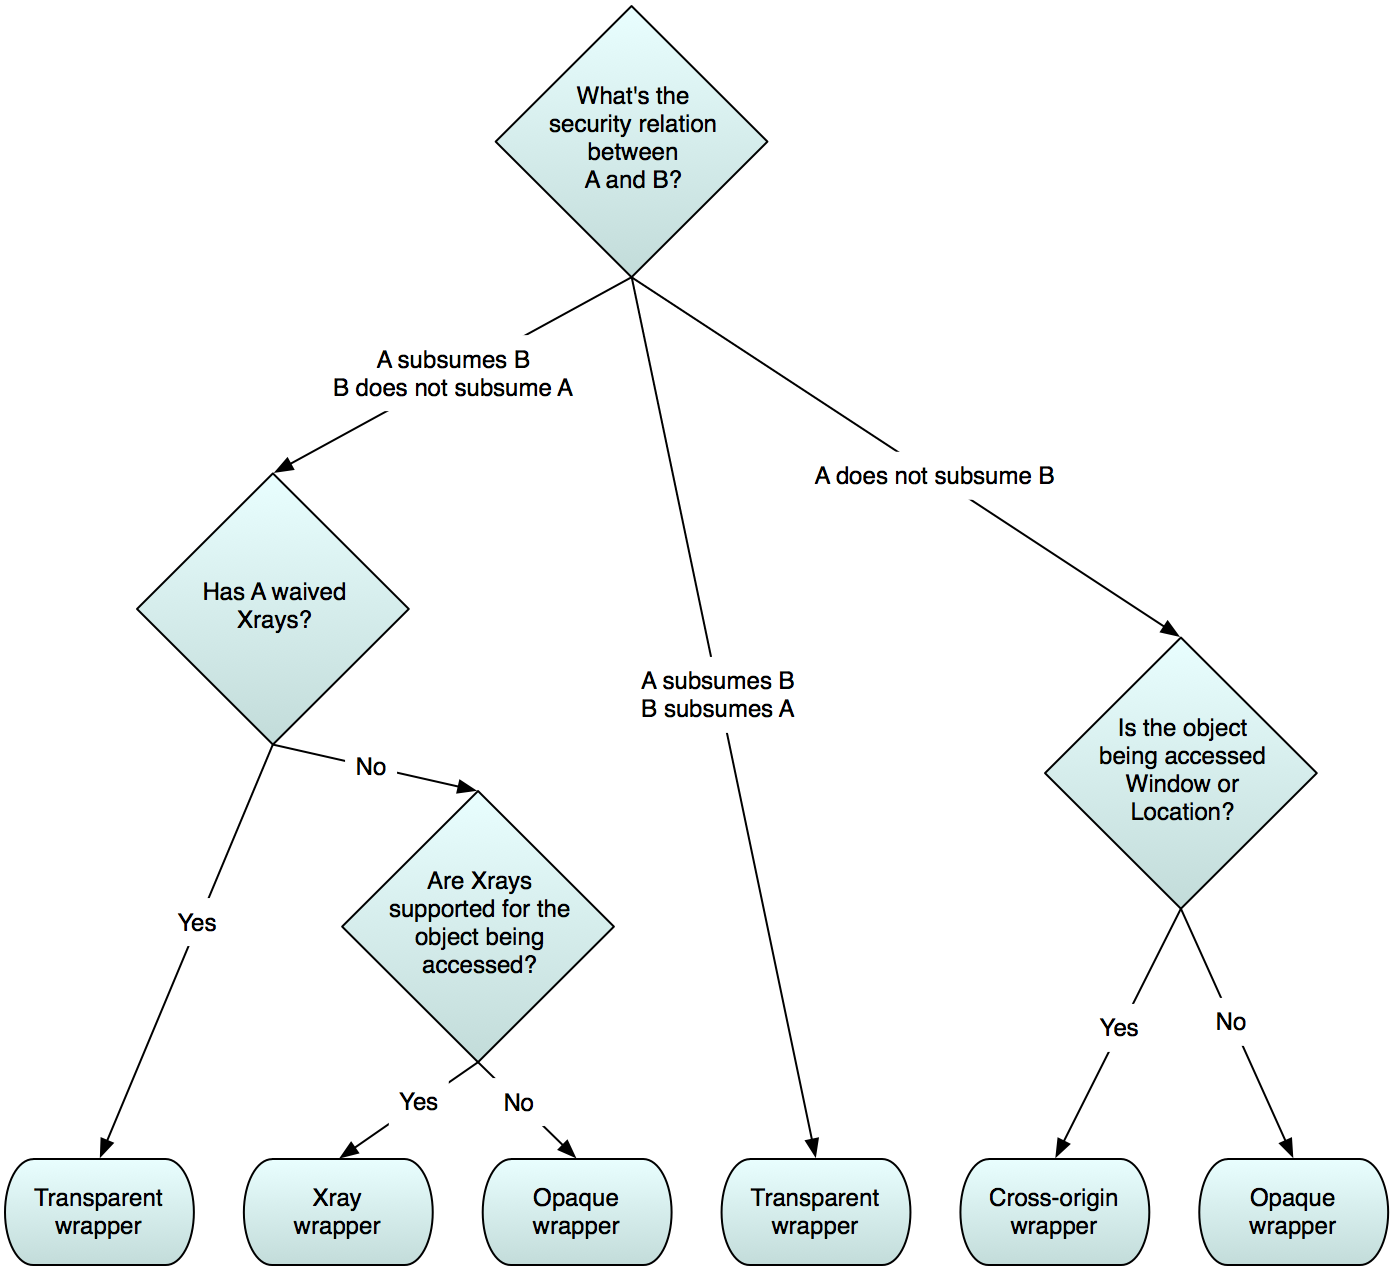
\includegraphics[width=0.5\textwidth]{computing-a-wrapper}  %% il file si chiama "computing-a-wrapper", larga 0.5 volte la largezza del testo
                \caption{Computare un wrapper}                              %% sotto l'immagine c'è una linea descrittiva
                \label{fig:computing-a-wrapper}                             %% potrà essere referenziata da link del documento con questo nome
            \end{figure}

        \subsection{Xray Vision}
        \label{sec:sicurezza-xray-vision}
            Javascript è un linguaggio molto malleabile il che lo rende imprevedibile in una contesto di
            sicurezza, oggetti provenienti da compartimenti insicuri potrebbero venire adeguatamente
            modificati per ingannare gli script privilegiati ad eseguire codice malevolo; per arginare
            il problema Gecko fa uso dei wrapper Xray, che consentono accesso completo alla forma "base"
            dell'oggetto ignorando le modifiche attuate dagli script, il modo in cui viene ottenuta
            dipende dall'oggetto acceduto.\\
            Gli elementi del DOM sono gli oggetti piu comuni e hanno due implementazioni: 
            una a livello Javascript che "vive" all'interno del proprio compartimento e memorizza lo
            stato corrente dell'oggetto, e una in codice nativo C++ che descrive la forma base
            dell'oggetto, quando il codice privilegiato deve accedere ad un elemento del DOM, gli viene
            restituito un wrapper Xray che mostra le proprietà della rappresentazione nativa. 
            Alcuni oggetti esistono solo nel runtime Javascript, come gli \code{Array} o le \code{Promise},
            allora si restringono le loro proprietà trattandoli come dizionari: metodi, getter e setter 
            sono ignorati per impedire l'esecuzione di codice malevolo mentre il prototype di \code{Object}
            e \code{Array} viene rimpiazzato con il prototipo standard garantendo l'integrità.\\
            Semmai il codice privilegiato avesse bisogno di conoscere lo stato corrente dell'oggetto la
            visione Xray può venire attenuata programmaticamente accedendo alla prorpietà \code{.wrappedJSObject},
            ma a questo punto non si avrebbero piu garanzie di sicurezza su di esso, nè sui "figli".


\chapter{WebExtension nel dettaglio}
\label{cap:webextension-dettaglio}
    Il codice del WebExtension framework può essere trovato nella cartella \file{toolkit/components/extensions/}, è composto
    da molti file che suddividerò in tre categorie: core, integrativi ed implementativi.\\
    I file di \bold{core} definiscono logica e strutture in ambiente nativo che verranno indirettamente utilizzate da
    tutti gli altri file, eseguono a livello di processo e svolgono ruoli di gestione della comunicazione tra
    processi e avviamento degli altri script.\\
    I file detti \bold{integrativi} definiscono la logica del framework, sono perlopiù moduli \JS
    e lavorano a stretto contatto con i servizi e le utilities fornite da Gecko, come contesti di esecuzione \JS, sandbox, storage
    e cache. Il loro compito è di gestire i dati delle estensioni nel Content Process ospite e sincronizzare le strutture
    di rappresentazione dell'estensione collocate sugli altri processi; per queste ragioni troviamo classi che
    coordinano l'invio e la ricezione di chiamate a procedure remote, classi per il setup e l'avviamento
    del contesto \JS in cui verrà eseguita l'estensione, parsing dei manifesti e degli schemi implementativi
    che descrivono gli api.\\
    Infine gli script \bold{implementativi} definiscono gli oggetti che l'api espone, ovvero quelli ospitati
    dall'oggetto \code{browser} menzionato nella \Sezione{webextension-api}. Curiosamente le definizioni di tali
    oggetti non sono note al framework a tempo di compilazione, ma vengono introdotte a runtime dal framework stesso attraverso
    schemi \json che contengono metadati sugli api e referenze ai rispettivi script \cite{webextension-api-development}, infatti i file cosiddetti implementativi
    sono schemi \json (indicizzati da \file{ext-toolkit.json} e collocati nella sottocartella \file{schemas/}) e script \JS
    che contengono il codice degli api esposti (residenti nelle sottocartelle \file{parent/} e \file{child/}).
    In questo capitolo illustrerò nel dettaglio i processi di gestione delle estensioni a runtime. \todo{continua, illustra il capitolo}

    \section{XPCOM}
        XPCOM Framework è un ambiente di sviluppo multi piattaforma che astrae elementi del sistema operativo,
        come la gestione della memoria, passing di messaggi e memoria condivisa, e fornisce interfacce di 
        comunicazione tra linguaggi programmazione; è il collante fondamentale tra i processi e le componenti di
        Gecko. Tra le feature di XPCOM il sottosistema XPConnect offre un linguaggio per definire
        interfacce di programmazione chiamato \idl ( Interface Definition Language ) e un linguaggio per definire protocolli
        di comunicazione inter-processo ed RPC chiamato \ipdl (Inte-process comunication Protocol Definition Language);
        il file di definizione, sia esso \idl o \ipdl, viene compilato in rappresentazioni equivalenti nei linguaggi
        di destinazione mentre la logica è implementata dal programmatore usando uno dei linguaggi specificati,
        al momento XPConnect supporta C++, Rust, Python, Javascript e pochi altri, tutti impiegati nello sviluppo
        di Gecko.\\
        Voglio aprire una parentesi di approfondimento su \ipdl per fare chiarezza sul concetto di \textit{Attore}, 
        menzionato nelle sezioni successive. A differenza delle interfacce un protocollo ha bisogno di due entità,
        dette Attori, che utilizzino il protocollo per un fine di comunicazione, \ipdl si riferisce ad essi come 
        Parent e Child. Il Parent viene collocato sul processo che rimarrà attivo più a lungo, idealmente il genitore, 
        mentre il Child è l'entità corrispondente attiva su un altro processo, idelamente figlio del primo.
        Durante la compilazione, XPConnect genera sia le strutture di rappresentazione dei protocolli che le
        interfacce di programmazione per gli attori, implementate allo stesso modo delle interfacce \idl.



    \section{ Loading }
        La vita di una estensione è legata a due classi: \AddonManager ed \ExtensionProcessScript,
        la prima è una classe singleton collocata nel Parent Process e responsabile della archiviazione
        degli Addon e delle estensioni ( prima di supportare lo standard WebExtension, Firefox veniva espanso
        usando gli Addon, \AddonManager è stata modificata successivamente per adattarsi al nuovo standard; quella degli
        Addon è una storia affascinante che si intreccia con l'evoluzione del sistema di sicurezza del browser ).
        Quando una estensione viene installata è \AddonManager a prendersi carico del collezionamento dei nuovi
        script nel database e di avviarli per la prima volta mentre il browser è in esecuzione; ma se \AddonManager
        è situata nella memoria del Parent Process come può iniettare uno script su altri processi isolati?
        \ExtensionProcessScript è un'altra classe singleton attiva su ogni Content Process, è incaricata di
        ottenere i dati e il codice delle estensioni e farne il setup preparandoli per il successivo utilizzo;
        inoltre è indirettamente responsabile dell'avvio all'interno del processo. Per rappresentare l'estensione
        \ExtensionProcessScript istanzia un oggetto \WebExtensionPolicy che ha la duplice funzione di astrarre
        l'estensione stessa e le informazioni di sicurezza associate tra cui l'entità di sicurezza,
        la Content Security Policy, l'Origin e altre proprietà interne; tutti gli oggetti menzionati sono
        descritti da interfacce \idl ed implementati in codice nativo, eccetto \code{mozIExtensionProcessScript.idl}
        scritto direttamente in Javascript.
         
    \section{}


    \section{L'estensione a runtime}
        //
    
    \section{L'api a runtime}
    \label{sec:webextension-api-rpc}
        \todo{Come viene creato l'ambiente di esecuzione dell'api?}
        \todo{come viene invocata una funzione?}
        \todo{come si ottiene il valore di ritorno?}

    \section{Le difese delle estensioni}
        Nel \Capitolo{cap:infrastruttura-sicurezza-firefox} ho discusso il sistema di sicurezza generale
        degli script in Firefox, in questa sezione si mostreranno le difese specifiche dell'ambiente
        WebExtension. Consci dei rischi dietro l'abuso del WebExtension API, gli sviluppatori mozilla
        hanno cercato di ridurre al minimo le feature accessibili alle estensioni facendo una
        distinzione netta fra gli script che interagiscono con il browser e gli script che interagiscono
        con le pagine.

        \subsection{I content script}
        \label{sec:difese-content-script}
            In Manifest V2 i content script non hanno Content Security Policy, mentre in Manifest V3 sono soggetti
            alla CSP di default delle estensioni \refSection{sec:difese-background-sidebar}.
            A differenza dei background script il loro codice è ospitato in ogni
            \todo{in \refChapter{cap:infrastruttura-sicurezza-firefox} aggiungere sezione su Window context e browsing context }Window Context 
            che veda la propria origine tra le origini specificate nella voce \code{"matches"} del \manifest dell'estensione.
            La figura \ref{fig:vuln-manifest-contentscript} è un esempio di quanto detto,
            la voce \code{"content\_scripts"} è una lista di configurazioni dei content script introdotti dall'estensione,
            l'esempio dichiara un content script \file{content/csMain.js} che deve eseguirsi su tutte le
            origini che rispettano le espressioni regolari della voce \code{"matches"}.

            \begin{figure}[ht]
                \centering
                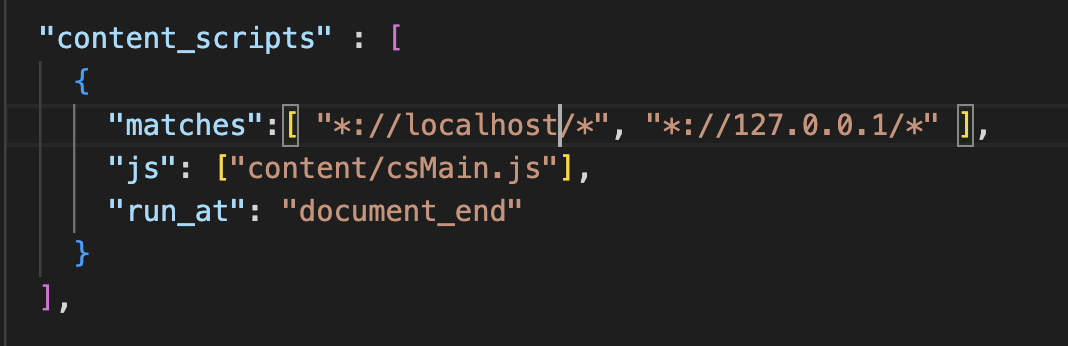
\includegraphics[width=0.85\textwidth]{vuln-manifest-content-script.png}
                \caption{Sezione content\_scripts nel \manifest di \vuln}
                \label{fig:vuln-manifest-contentscript}
            \end{figure}

            I content script possono accedere ad un insieme ristretto di WebExtension API, perlopiù event listener,
            servizi di messaging, conversione dei locales e storage.

        \subsection{I background script e la sidebar}
        \label{sec:difese-background-sidebar}
            Sugli script di background e le UI viene applicata una CSP di default modificabile soltanto dal
            \manifest dell'estensione, i dettagli della policy differiscono tra Manifest V2 e V3. Nella
            mia ricerca ho trattato solo la versione 2 del manifest pertanto tratterò solo le specifiche
            di quest'ultima.
            La CSP di background è piu severa rispetto ai content script volta a restringere le origini
            da cui caricare codice \JS e pratiche di programmazione potenzialmente insicure, la specifica
            standard del manifest V2 è:
            \begin{lstlisting}
                "script-src 'self'; object-src 'self';"
            \end{lstlisting}
            Nel pratico la riga precedente si traduce in quattro restrizioni:
            \begin{itemize}
                \item Risorse \code{<script>} e \code{<object>} possono essere caricate solo da origini
                        locali all'estensione (ovvero file collocati nella stessa cartella). Tutte le
                        richieste che cercheranno di includere codice nella pagina proveniente da origini
                        considerate insicure verranno bloccate silenziosamente.

                \item Non è concesso evaluare stringhe come codice \JS. L'uso di funzioni come
                        \code{eval()}, \code{setTimeout()}, \code{setInterval()} e \code{Function()}
                        per eseguire il contenuto di stringhe come codice \JS viene bloccato silenziosamente.
                
                \item Non è consentito eseguire codice \JS inline. Con codice inline si intende codice
                        \JS hard-coded in elementi html, come quello contenuto nel tag \code{<script>}
                        quando non viene utilizzato per includere file script. Un esempio è l'abuso degli
                        event listener dichiarabili direttamente sui tag html per eseguire \JS malevolo:\\
                        \code{<img src="invalid" onerror=fetch("http://attacker/?" + document.cookie) >}        

                \item \todo{due parole su webassembly} Non è consentito eseguire codice WebAssembly.
            
            \end{itemize}
            Questa politica è applicata su ogni estensione che non abbia esplicitamente modificato la voce
            \code{"content\_security\_policy"} del suo \manifest e non è modificabile programmaticamente.
            
        \todo{forse questa sezione dovrebbe stare in \refChapter{cap:webextension-dettaglio} }\subsection{API}
        \label{sec:difese-api-sandbox}
            L'implementazione del WebExtension API è collocata nel Parent Process all'interno
            di una Sandbox che esegue come Entità di Sistema \refSection{sec:security-principal} ed ha
            accesso a molti servizi del browser (vedi \file{ExtensionCommon.sys.mjs} \method{\_createExtGlobal}).


\chapter{Analisi di \vuln}
\label{cap:analisi-vuln}
    Questo capitolo illustra gli script e le componenti che verranno abusate dagli attacchi
    discussi nel \refChapter{cap:attaccando-vuln}.
    La \refSection{sec:analisi-vuln-manifest} tratta l'analisi del manifest, file di presentazione
    sia per le estensioni che per questo capitolo,
    a seguire la \refSection{sec:analisi-vuln-sidebar} discuterà del codice dietro la sidebar
    di \vuln e le istruzioni responsabili di aver introdotto la vulnerabilità nell'estensione,
    infine nella \refSection{sec:analisi-vuln-content-script} si mostra il codice del
    content script che giocherà un ruolo chiave durante gli attacchi.

    \section{Il \manifest}
    \label{sec:analisi-vuln-manifest}
        Ora che l'ambiente WebExtension è stato discusso approfonditamente è il momento di
        osservare una estensione fatta e finita e comprendere se frammenti di codice vulnerabile
        possano costituire realmente una minaccia per l'utente che l'ha installata.
        L'analisi incomincia dal \manifest dell'estensione riportato nel listato seguente:
        \begin{lstlisting}
    {
        "manifest_version": 2,
        "name": "vuln",
        "version": "1.0",
        "description": "vuln",

        "content_scripts" : [
            {
            "matches":[ "*://localhost/*", "*://127.0.0.1/*", "*://www.attacker.xyz/*" ],
            "js": ["content/csMain.js"],
            "run_at": "document_end"
            }
        ],

        "sidebar_action": {
            "default_title": "Vuln sidebar",
            "default_panel": "sidebar/page.html"
        },

        "background" : {
            "page": "background/bgPage.html",
            "persistent": false
        },

        "permissions": [
            "storage"
        ]
    }
        \end{lstlisting}
        Gia dalla prima voce otteniamo una informazione importante, si tratta di un Manifesto Versione 2,
        questo significa che i content script non saranno soggetti a restrizioni di Content Security Policy.
        La voce \code{"content\_scripts"} di \vuln dichiara un solo content script attivo su qualsiasi pagina ospitata dalla
        lista \code{"matches"} di pattern d'origine, i tre pattern di \vuln sono da interpretare come:
        \textit{"qualsiasi porta e qualsiasi protocollo sui domini localhost, 127.0.0.1 e www.attacker.xyz"},
        il codice dello script si strova nel file \file{content/csMain.js} e deve essere eseguito
        alla fine del caricamento della pagina (voce \code{"run\_at"}), probabilmente perché avrà bisogno
        di accedere ad elementi del documento html, elementi che devono avere il tempo di essere caricati.
        La voce \code{"sidebar\_action"} dichiara che l'estensione intende aggiungere un pannello di sidebar
        che visualizza il documento \file{sidebar/page.html} il cui fine è ancora ignoto, analogamente
        il browser dovrà ospitare anche una finestra in background \file{background/bgPage.html}, entrambe
        queste finestre avranno accesso all'api \code{"storage"} come indicato nell'ultima voce \code{"permissions"};
        pertanto è lecito supporre che almeno una di esse ospiti codice \JS e memorizzi dati nello storage.
        

    \section{La sidebar}
    \label{sec:analisi-vuln-sidebar}
        Come detto nella \refSection{sec:estensione-vuln}, per costruzione sappiamo gia che la vulnerabilità
        risiede nella logica della sidebar. I listati seguenti mostrano rispettivamente il codice html del documento
        visualizzato nella sidebar e lo script che ne determina il comportamento:

        \begin{lstlisting}[caption={Contenuto di \file{sidebar/page.html}},captionpos=b,label=code:sidebar/page.html]
<!doctype html>
<html>
  <head>
    <meta charset="utf-8" />
    <link rel="stylesheet" href="page.css" />
    <script src="../shared/archive.js"></script>
    <script defer src="sbMain.js"></script>
    
  </head>

  <body>
    <p>Archive:</p><br/>
    <section id="output"></section>
  </body>
</html>
        \end{lstlisting}

        \begin{lstlisting}[caption={Contenuto di \file{sidebar/sbMain.js}},label=code:sidebar/sbMain.js]

const output = document.getElementById("output");

function updateArchiveView(arch) {

    output.innerHTML = "";

    for ( let data of arch ) {
        let container = document.createElement("div");
        let keyField = document.createElement("span");
        let valField = document.createElement("span");
        let br = document.createElement("br");

        keyField.innerHTML = data.key + ": ";
        valField.innerHTML = data.value;

        container.appendChild( keyField );
        container.appendChild(valField);
        container.appendChild(br);

        output.appendChild(container);
    }
}

function main() {
    getArchive()
    .then( updateArchiveView );

    addArchiveChangeListener( (storage) => { updateArchiveView(storage[ARCHIVE_NAME].newValue) } );
}

window.onload = main
        \end{lstlisting}

        Il codice della pagina non contiene informazioni rilevanti eccetto gli script inclusi
        a righe 6 e 7. \file{../shared/archive.js} è uno script di utility sul quale non mi soffermerò, basti sapere
        che dichiara le funzioni \code{getArchive()} e \code{addArchiveListener()}, rispettivamente
        per ottenere l'archivio di storage e registrare un listener richiamato al cambiamento dei
        dati nello storage, mentre \file{sbMain.js} è lo script dietro al comportamento della
        pagina. La sua logica è semplice: la funzione \code{updateArchiveView()} ottiene in input
        una lista di oggetti contenenti una coppia \code{key} e \code{value}, per ogniuno di essi
        inserisce nel documento due elementi html \code{<span>} che mostrano il valore di \code{key}
        e \code{value} rispettivamente; \code{updateArchiveView} viene invocata al caricamento
        della finestra e ogni volta che l'archivio è modificato. A righe 14 e 15 della funzione 
        si trova la vulnerabilità, l'assegnazione diretta dei valori all'attributo \attr{innerHTML}
        degli elementi \code{<span>}.\\
        Seppure appaia come attributo, la proprietà \attr{innerHTML} è in realtà una coppia di metodi
        getter/setter, quando si assegna un valore viene richiamato il metodo setter che inserisce
        il valore tra il tag iniziale e terminale dell'elemento modificato come codice html valido
        che verrà eseguito all'inserimento nella pagina. Di conseguenza se \code{key} o \code{value}
        dovessero essere stringhe contenenti sintassi html allora verrebbero eseguite aprendo la
        strada a una possibile compromissione della pagina, ma da dove provengono i valori della
        coppia?

    \section{Il content script}
    \label{sec:analisi-vuln-content-script}
        Dal punto di vista del sistema di sicurezza il codice del content script è considerato
        una Entità Estesa (vedi \refSection{sec:security-principal}) che ha come oggetto
        globale la \code{window} della pagina web su cui sta venendo eseguita, la quale
        però è una Entità di Contenuto; pertanto secondo la Security Policy di Firefox (vedi \refSection{sec:sicurezza-script-security-policy})
        i content script hanno una visione ridotta degli oggetti del DOM (vedi \refSection{sec:sicurezza-xray-vision}).
        Per avere visione delle proprietà reali il content script deve mitigare lo strato
        di sicurezza e ottenere l'oggetto sottostante, a questo serve l'attributo \attr{wrappedJSObject},
        richiamabile dagli script su oggetti collocati in compartimenti meno "privilegiati".
        Terminato il preambolo, ecco riportato il codice \JS dietro al content script di \vuln:
        \begin{lstlisting}

const getPayload = ( obj ) => {

    if ( obj instanceof Document ) {
        // Cerca Elementi "key" e "value" nel document
        obj = obj.wrappedJSObject;
        return { 
            key: obj.getElementById("key")?.innerHTML, 
            value: obj.getElementById("value")?.innerHTML 
        };
    }
    else if ( obj instanceof Event ) {
        // Cerca attributi "key" e "value" nei dettagli dell'evento custom
        obj = obj.wrappedJSObject;
        return {
            key: obj.detail.key,
            value: obj.detail.value,
        }
    }
    else
        throw new Error("Cannot recover payload from this object");
}


window.addEventListener( "trigger", (ev) => {
    const payload = getPayload( ev );
    payload && browser.runtime.sendMessage( payload );
} )

window.onload = () => {
    const payload = getPayload( document )
    payload && browser.runtime.sendMessage( payload );
}

        \end{lstlisting}
        La funzione \code{getPayload} definita nelle prime righe del file estrapola la coppia
        \code{key} \code{value} dall'oggetto passatogli come argomento che può essere istanza
        di un documento DOM o di un evento. Se si tratta di un documento allora i dati vengono
        cercati nel contenuto della pagina come testo html racchiuso rispettivamente nel corpo
        degli elementi \code{key} e \code{value}; invece se l'oggetto è un evento allora i
        dati sono estrapolati dal suo campo \attr{detail}. In entrambi i casi la visione Xray
        deve essere disattivata.
        Infine il ritrovamento della coppia viene notificato al runtime e i dati inviati come
        corpo del messaggio, successivamente lo script di background li immagazzinerà nello
        storage per poter essere letti e visualizzati dalla sidebar.\\
        Sui dati non viene fatto alcun controllo né sul tipo, né sul contenuto né sulla loro
        integrità percui il codice della sidebar non ha modo di sapere se le stringhe che sta
        inserendo nella propria finestra contengano sequenze di caratteri potenzialmente malevoli.


\chapter{Attaccando \vuln}
\label{cap:attaccando-vuln}
    si insomma dopo tutta sta trafila giungiamo ai fatti.


\chapter{Conclusioni}


\printbibliography


\end{document}
%% END ARTICOLO